\chapter*{Appendix}
\addcontentsline{toc}{chapter}{Appendix}

\section{Story - AITA for telling my roommate her sister has to pay rent?}\label{text:story}
So I got an apartment with my best friend 1.5 years ago and it has been a rocky relationship ever since. We literally go weeks without talking. Last year she let a friend crash on the couch for months and he only split the bills one time in like six months. I later found out that he was actually just splitting her half of the bills with her. I later found out he was in fact paying bills but he was splitting her half of the bills. Our rent is \$600 a month and instead of all of us paying \$200. i paid \$300 and they each paid \$150. I felt that was unfair seeing how he was sleeping in the living room and I could no longer access it and it inconvenienced me but it didn’t matter anymore because I didn’t find out until after he moved out. Now she has told me her sister will be moving in due to family issues and I told her head on we should split the bills 3 ways since she’s sleeping in the living room \& not sharing the room with my roommate. She feels that her sister should only split her half with her since she’s “her responsibility \& company.” AITA for telling her that her sister has to split the bills evenly or she can’t stay in the living room?
[This is the original Reddit story. The story is told in Portuguese on the videos.]

\clearpage
\section{Pre Questionnaire}
\begin{figure}[h!]
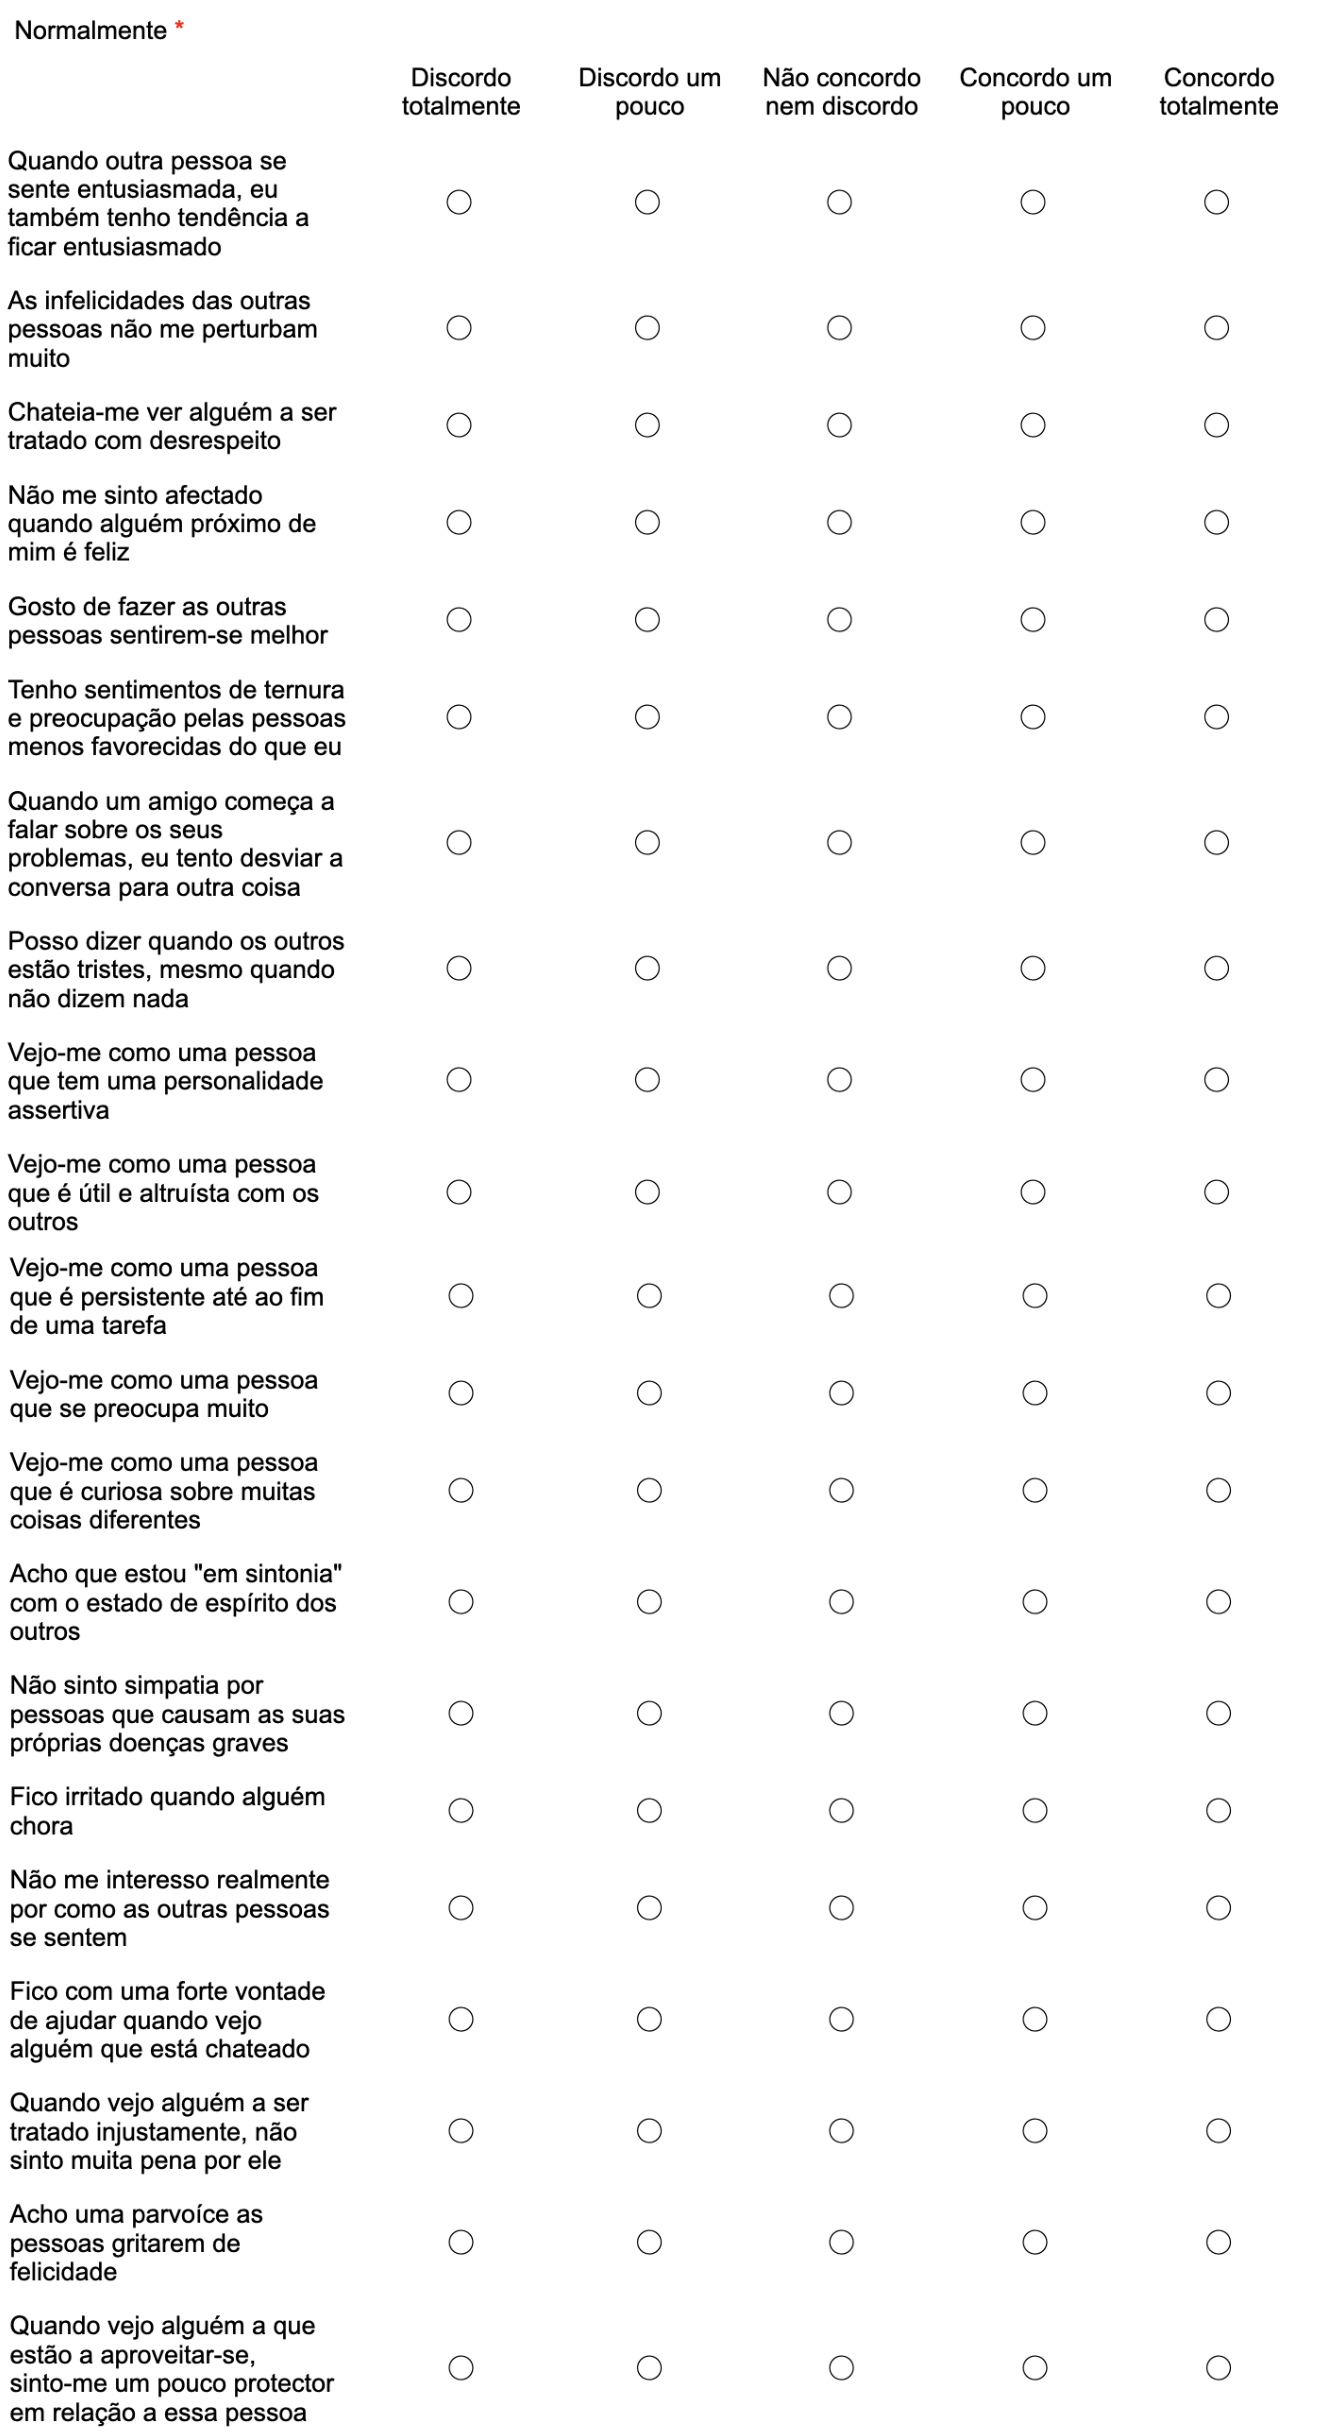
\includegraphics[scale=0.25]{figures/pre.png}
\centering
\label{fig:pre}
\end{figure}

\clearpage
\section{Post Questionnaire - Pre-recorded videos}
\begin{figure}[h!]
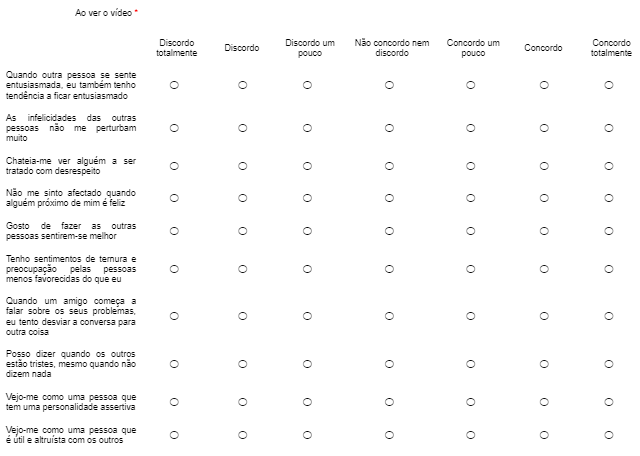
\includegraphics[scale=0.65]{figures/post.png}
\centering
\label{fig:videoPost}
\end{figure}

\clearpage
\section{Post Questionnaire - Transcript}
\begin{figure}[h!]
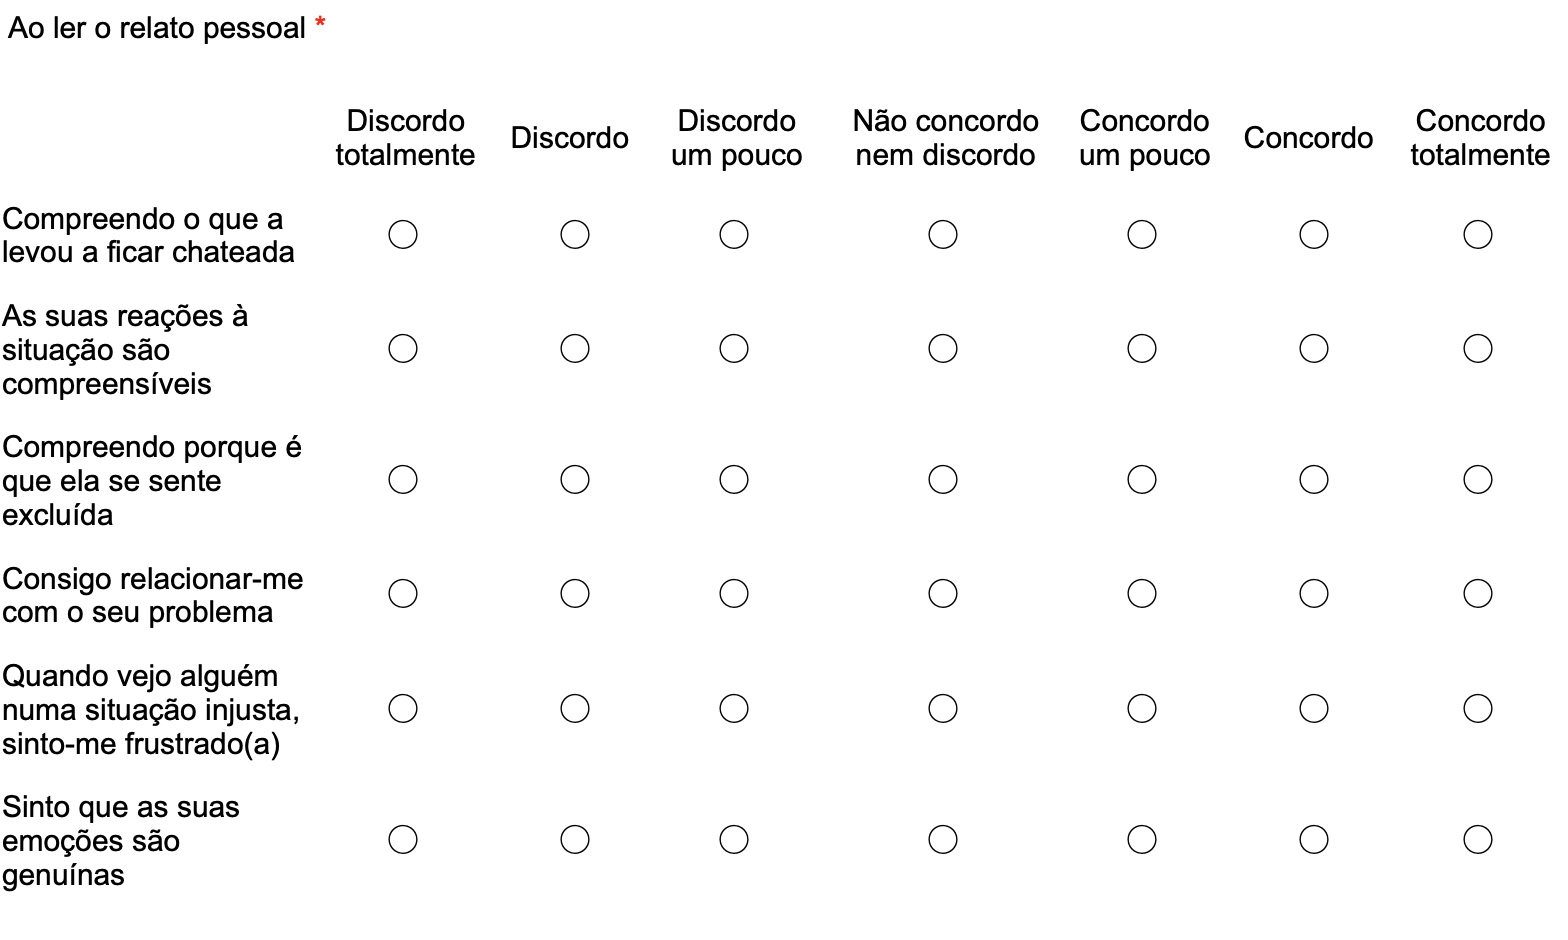
\includegraphics[scale=0.6]{figures/postTranscript.png}
\centering
\label{fig:transcriptPost}
\end{figure}